\documentclass[11p]{article}
% Packages
\usepackage{amsmath}
\usepackage{graphicx}
\usepackage{fancyheadings}
\usepackage[swedish,english]{babel}
\usepackage[
    backend=biber,
    style=authoryear-ibid,
    sorting=ynt
]{biblatex}
\usepackage[utf8]{inputenc}
\usepackage[T1]{fontenc}
\usepackage{titlesec}
\usepackage{hyperref}
%Källor
\addbibresource{references.bib}
\graphicspath{ {./images/} }

% Lite variabler
\def\email{levi.hogdal@ga.ntig.se}
\def\foottitle{Gymnasiearbete}
\def\name{Levi Högdal}

\title{Gymnasiearbete \\ \small Gymnasiearbete}
\author{\name}
\date{\today}

\begin{document}

% fixar sidfot
    \lfoot{\footnotesize{\name \\ \email}}
    \rfoot{\footnotesize{\today}}
    \lhead{\sc\footnotesize\foottitle}
    \rhead{\nouppercase{\sc\footnotesize\leftmark}}
    \pagestyle{fancy}
    \renewcommand{\headrulewidth}{0.2pt}
    \renewcommand{\footrulewidth}{0.2pt}

% i Sverige har vi normalt inget indrag vid nytt stycke
    \setlength{\parindent}{0pt}
% men däremot lite mellanrum
    \setlength{\parskip}{10pt}

    \maketitle
    \begin{center}
    
\includegraphics[width=0.4\textwidth]{../images/NTI Gymnasiet_Symbol_print_svart.png}
    \end{center}

    \newpage
    \begin{abstract}
        abstract
    \end{abstract}
    \newpage
    \tableofcontents
    \newpage

    \section{Inledning}
    Att kunna använda en hemsida på ett bra sätt är något många nuförtiden tar för givet.
    Att förstå internet och kunna enkelt läsa och navigera olika forum och hemsidor är inte något som personer som har använt internet.
    Det finns många olika sätt som en hemsida ska se utt och designas men hur ska hemsidor anpassas för folk som har svårt att använda internet.
    Om man har någon funktionsnedsättning eller om det är väldigt dålig kontrast på en hemsida så blir den svår att använda.
    För att underlätta så att allt inte är kaos och användaren ska kunna använda hemsidan på ett bra sätt har en organisation som heter W3C skapat standarder(WCAG) för användbarhet på hemsidor.
    Hur mycket hemsidor förhåller sig till WCAG standarden är varierande men jag är intresserad i hur olika kommunala hemsidor förhåller sig till dem.
    
    \subsection{Syfte och frågeställning}
    Det jag vill undersöka är:
    Vilka WCAG2.2 krav uppfyller kommuners hemsidor och vilka skillnader finns det i kraven som kommunerna uppfyller.
    Finns det några skillnader på invånare i kommunen och hur många krav kommunen uppfyller. [Kanske]

    \section{Bakgrund}

    \subsection{Tillgänglighet}
    Tillgänglighet i det här sammanhanget betyder inte hur åtkomligt något ska vara utom att saker ska kunna användas av alla personer även de med funktionsnedsättning.
    Tillgänglighet handlar om saker som hur bra kontrast det är mellan bakgrund och text så att det ska vara enkelt att läsa texten och har bilder en bildtext, inte kan jag komma åt hemsidan \parencite{webbriktlinjer}.
    Webbsidor design och utformning ska vara anpassad så att alla människor ska kunna använda och förstå hemsidan så länge de kan läsa språket.
    För att hemsidor ska se vettiga ut och användas av folk med funktionsnedsättningar så görs standarder som man kan följa när man skapar hemsidor och olika lagar.
    Webbstandarden som den här undersökningen kommer hålla sig till är WCAG som är utgivet av W3C.


    \subsection{Hemsidors uppyggnad}
    Hemsidor brukar vara uppbyggda i grunden av 4 olika delar:
    \begin{itemize}
        \item Hypertext markup language (HTML)
        \item Cascading style sheets (CSS)
        \item Accessible rich internet applications (ARIA)
        \item Javascript/Typescript (JS/TS)
    \end{itemize}
    Den här undersökningen är intresserad i HTML, CSS och ARIA men inte Javascript/Typescript.
    Javascript och Typescript är programmeringsspråk som används i bakgrunden av hemsidan för att programmera in funktioner som inte redan finns i HTML eller bestämma hur servern hanterar hemsidan på sin sida.
    WCAG krav handlar mest om användarens upplevelse av hur hemsidan fungerar och inte detaljerna på hur en hemsida fungerar.

    \subsubsection{Hypertext markup language}
    Hypertext markup language (HTML) är standardspråket som hemsidor är gjorda av.
    HTML är språket som ger struktur och definierar grunden till hur hemsidan ser ut \parencite{HTML}.
    Ett element är skriven på följande vis <body> och </body>.
    Den första <body> kallas för en öppnings tagg och är början av elementet och den andra </body> kallas för stängnings tagg och är slutet av elementet.
    Man kan också skriva mer i en tagg till exempel <article id="article"> där det första ordet är vilket element det är och den andra i det här fallet är ett id som kan användas för att hitta och interagera elementet med exempelvis javascript.
    En stängnings tag är alltid på följande vis: </p>, </body>, </main>, </head>, </div> och så vidare.
    Text som inte är i en tagg kommer att hanteras som normalt textinnehåll och skrivas up på hemsidan som normal text.
    I elementen ingår grundfunktioner och grundstilar som bestämmer hur texten kommer se ut och formateras när den skrivs ut på hemsidan.

    \subsubsection{Cascading style sheets}
    Cascading style sheets (CSS) är ett språk som används för att bestämma hur en hemsida ser ut \parencite{CSS}.
    Grundstilarna i HTML gör en hemsida som fungerar, inte en som ser bra ut.
    De estetiska

    CSS tillåter att ändra grundstilen på ett element till något annat.
    För att bestämma hur en hemsida ser ut grafiskt används CSS x

    Programmet WAVE som används i undersökningen och förklaras senare tillåter att stänga av "STYLE" vilket är css.

    \subsubsection{Accessible rich internet applications}
    Accessible rich internet applications (ARIA) är extra roller och attribut som används för att göra en hemsida mer tillgänglig.
    ARIA har mest funktionalitet om man inte navigerar hemsidan som en normal användare utan med andra hjälpmedel \parencite{ARIA}.
    Att implementera ARIA på ett felaktigt sätt gör en hemsida mindre användarvänlig och om det går bör man använda HTML element och attribut som gör samma saker.
    
    \subsection{The world wide web consortium}
    The world wide web consortium (W3C) är det företaget som var utgivarna WCAG 2.2 standarden som användes i undersökningen \parencite{W3C}.
    W3C är ett företag som grundades av Tim Berners-Lee med syftet att säkerställa webbens utveckling och framtid.
    För att uppnå målet har de skapa standarder för webben och har diskussioner med flertal grupper och organisationer om webben.
    WCAG standarden har de skapat och det är den som undersökningen kommer att utgå ifrån.

    \subsection{Web content accessibility guidelines}
    Web content accessibility guidelines (WCAG) är en lista av riktlinjer för webben \parencite{WCAG_2.2}.
    Målet med riktlinjerna är att göra webben mer tillgänglig och användarvänlig så att alla användare kan använda hemsidan.
    WCAG 2.2 är indelad i 4 stora kategorier och varje individuellt krav ska kunna testas separat.
    \\De olika delarna är:
    \begin{enumerate}
        \item Märkbart
        \item Manöverbart
        \item Begriplighet
        \item Robust
    \end{enumerate}

    Märkbart handlar om att information och innehåll ska vara synligt och tillgängligt för användare.
    Ljudbaserad media ska vara tillgängligt för användare som är döva.
    Den visuella presentationen av hemsidan ska vara läsbar och enkel att förstå.

    Manöverbart handlar att hemsidan ska vara navigerbar på ett användarvänligt vis.
    Det finns flera vägar än bara mus och tangentbord att navigera en hemsida och de behöver också fungera.
    Hemsidor ska till exempel vara navigerbar med pekskärmar och endast tangent.

    Begriplighet handlar om att användaren ska förstå innehållet på hemsidan.
    Att förstå innehållet på en hemsida är inte alltid det lättaste och det är ännu svårare om användaren har en funktionsnedsättning.
    Navigationen och språket på hemsidan ska vara tydligt och eventual fel som användaren gör ska förklaras.

    Robust relaterar till att olika program ska kunna bestämma vad innehåll betyder och gör.
    Semantisk mening i de olika elementen är viktiga för att program ska kunna tolka hemsidan på ett bra sätt.

    \subsubsection{Varför WCAG 2.2}
    WCAG är globalt sett den accepterade webbstandarden och om man kollar på lagar och regler som finns i sverige och EU ser man att det utgår från WCAG.
    I den svenska myndighetens kriterier för hur webbplatser ska användarvänlighets anpassas finns det direkt länkat till vilket WCAG som kravet utgår ifrån. \parencite{Utförande_av_Dos_lagen}
    Den här undersökningen utgår ifrån WCAG 2.2 vilket var den senaste version av WCAG standarden när undersökningen gjordes.


    \subsubsection{Varför är WCAG den globala standarden}
    Kan bara hitta resurser som säger att det är standarden och inte direkt varför det är standarden
    Är det bara att skriva att de var dom som först försökte skapa ordning och reda på webben och folk tyckte att deras krav och förslag var vettiga så man bara accepted det som den globala standarden.

    [förmodligen borde förklaras med W3C]

    \subsection{Lagar}
    I sverige finns en lag som heter "Lagen om tillgänglighet till digital offentlig service (DOS-lagen)".\parencite{Dos-lagen}
    Lagen ställer krav på offentliga aktörer så att de ska tillgänglighetsanpassa webbplatser och mobila applikationer.
    Myndigheten för digital förvaltning (Digg) är ansvarig för att genomföra lagen och de utgår från WCAG standarden för att sätta krav på hemsidorna.

    \subsubsection{Offentlig aktör}
    Hur en offentlig aktör definieras finns förklarat i \textcite{Dos-lagen} men det kan enklare förklaras som offentlig information från staten som statliga och kommunala myndigheter samt sammanslutningar till dem.
    Saker som rör utbildning, skola, sjukvård ock omsorg måste också följa lagen.
    Även om det ägs privat så kommer de behöva följa kraven från Dos-lagen.

    Det kan enklare förklaras som statliga och kommunala myndigheter, beslutstagande församlingar i kommuner och regioner, skola och sjukvård.\parencite{Om_Dos-lage}


    \subsection{Verktyg}
    För att underlätta min undersökning användes 2 digitala verktyg.
    Det första heter web accessibility evaluation tools (WAVE).
    WAVE är en webbtillägg och hemsida som tillåter automatiskt testning för några WCAG krav \parencite{WAVE}.
    WAVE kollar kontrasten på innehållet, redovisar HTML strukturen och vart ARIA används på hemsidan.
    Fell i HTML syntax redovisas enkelt och ikoner på hemsidan visas var olika element och attribut används.

    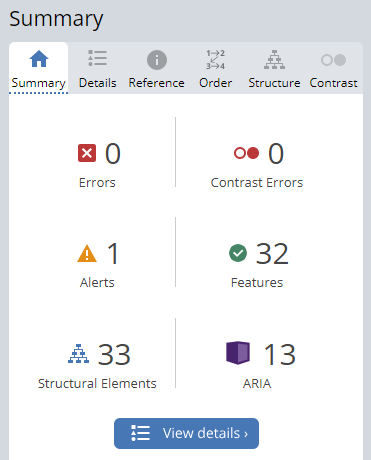
\includegraphics[width=0.4\textwidth]{../images/WAVE.png}

    WAVE resultatet från sorsele kommun startsida.

    Det andra verktyget är en screen reader.
    En screen reader läser upp ett html element och dess textinnehåll.
    Det finns WCAG krav där användaren programmässigt sätt ska kunna bestämma vad något är och vad det har för funktion.
    Till exempel finns WCAG krav 1.3.5 Identify Input Purpose (Level AA) där användaren ska kunna bestämma vilken information ett textinmatningsfält ska få in.
    Med en screen reader ska den berätta för användaren att det är ett textinmatningsfält och vilken information som ska in.

    \subsection{Komunala Hemsidor}
    För att meddela information om en kommun digital har kommuner hemsidor som det styr innehållet på och lägger upp information om kommunen.
    Det som är intressant om kommunal hemsidor är att alla är inte bara en hemsida som ser lika dan ut för varje kommun utan de ser annorlunda ut men vissa kommuner har hemsidor som ser likadana ut bara varierande innehåll.
    Skillnaden i hur kommunala hemsidor ser ut betyder att det finns en skillnad på hur de är uppbyggda och hur det är anpassade för användarvänlighet för webben.
    
    Hemsidorna i undersökningen valdes från listan på \textcite{SverigesKommuner}.
    Listan var ordnad i folkmängd störst till mins för alla kommuner i sverige.
    
    \section{Metod och Material}

    Undersökningen utgick på att testa hur om kommunernas hemsidor uppfyller alla krav i WCAG 2.2.
    Digg och W3C har givit ut en listor över hur kraven kan uppnås i lagen och WCAG 2.2.
    För specifikation om WCAG kraven se \textcite{WCAG_2.2}
    Undersökningen utgick ifrån en sammanställning över kraven och hur de kan mötas i ett kalkylark (se bilaga 1).
    Utifrån den tabellen testades alla kraven på hemsidorna.
    Nedan fins en förklaring av vad varje colum i tabellen består av.
    \begin{enumerate}
        \item Själva WCAG 2.2 kravet som skulle testas.
        \item Hur WCAG 2.2 kravet ska testas
        \item På vilken hemsida som kravet testades
        \item Om hemsidan uppfyllde kravet
        \item Kommentarer om hemsidan
        \item 3-5 repeterade 2 gånger till för att få plats för 2 hemsidor till.
    \end{enumerate}

    \section{Resultat}

    På alla hemsidor så testades inte 16 av de 86 kraven.

    Det finns 3 krav som inte testades för att jag inte hade en bra väg att kunna testa dem.
    Krav 2.2.5 Re-authenticating (Level AAA) vilket handlar om att användaren loggar in igen efter den har blivit utloggad utan dataförluster.
   \\ Krav 3.3.4 Error Prevention(Legal, Financial, Data) (Level AA) vilket handlar om förbyggande av fel vid finansiella transaktioner och lagligt bindande kontrakt.
    Till exempel att informationen ska kollas efter fel när användaren skriver in information för att köpa något.
  \\  Krav 3.3.6 Error Prevention (All) (Level AAA) vilket är typ samma som 3.3.4 fast det är inte restrikterat till finansiella transaktioner och kontrakt.
    All information som användaren skickar in ska kollas efter fel och användaren ska kunna åtgärda de felen.

    11 av kraven inom den första kategorin av märkbart testades inte.
    Kraven handlade om ljud och innehåller saker som att det ska finns undertexter och teckenspråkstolkning för videor och ljud med mera.
    De testades inte av den enkla anledningen av att jag inte hittade någon ljudfil eller videofil på hemsidan.

    Krav 2.1.4 Character Key Shortcuts (Level A) handlar om tangentbordsgenvägar och testades inte för jag är inte medveten om några tangentbordsgenvägar på hemsidan.

    Krav 2.2.4 Interruptions (Level AAA) handlar om att sidan uppdateras i nutid med ny information.
    Det kravet testades inte för hemsidan hade inga delar som uppdaterades i nutid.

  \\  I slutändan testades 70 av de 86 kraven på hemsidorna.

    \subsection{Märkbart krav}
    I den första delen av WCAG märkbart finns 29 krav var 18 av de kraven testades.
    Sorsele kommun mötte 10 av de kraven och misslyckades med 8 av dem.
    Totalt lyckades kommunen med 55.56$\%$ av märkbart kraven.
    \\Höörs kommun mötte 13 av de kraven och misslyckades med 5 av dem.
    Totalt lyckades kommunen med 72.22$\%$ av märkbart kraven.
    \\Linköpings kommun mötte 14 av de kraven och misslyckades med 4 av dem.
    Totalt lyckades kommunen med 77.78$\%$ av märkbart kraven.
    \\I den här kategorin ligger sorsele kommun klart lite bakom de andra kommunerna medans linköping och höörs kommun skiljer det endast 1 krav.

    \begin{center}
    Märkbart krav (18 av 29 krav testades)

    \begin{tabular}{ |c|c|c|c|}
        \hline
        Kommun & möter & Möter inte & Möter ($\%$) \\  \hline
        Sorsele & 10 & 8 & 55.64$\%$ \\ \hline
        Höör & 13 & 5 & 72.22$\%$ \\ \hline
        Linköping & 14 & 4 & 77.78$\%$ \\ \hline
    \end{tabular}
    \end{center}

    \subsection{Mönöverbar krav}
    I den andra delen av WCAG manöverbar finns 34 krav var 31 av de kraven testades.
    Sorsele kommun mötte 21 av de kraven och misslyckades med 10 av dem.
    Totalt lyckades kommunen med 67.74$\%$ av manöverbar kraven.
    \\Höörs kommun mötte 30 av de kraven och misslyckades med 1 av dem.
    Totalt lyckades kommunen med 96.77$\%$ av manöverbar kraven.
    \\Linköpings kommun mötte 30 av de kraven och misslyckades med 1 av dem.
    Totalt lyckades kommunen med 96.77$\%$ av manöverbar kraven.
    \\Även i den här kategorin ligger sorsele bakom med Linköping och höörs kommun möte lika många krav.

    \begin{center}
    Manöverbar krav (31 av 34 krav testades)

    \begin{tabular}{ |c|c|c|c|}
        \hline
        Kommun & möter & Möter inte & Möter ($\%$) \\  \hline
        Sorsele & 21 & 10 & 67.74$\%$ \\ \hline
        Höör & 30 & 1 & 96.77$\%$ \\ \hline
        Linköping & 30 & 1 & 96.77$\%$ \\ \hline
    \end{tabular}
    \end{center}

    \subsection{Begriplighet krav}
    I den tredje delen av WCAG begriplighet finns 21 krav var 19 av de kraven testades.
    Sorsele kommun mötte 16 av de kraven och misslyckades med 3 av dem.
    Totalt lyckades kommunen med 84.21$\%$ av begriplighets kraven.
    \\Höörs kommun mötte 17 av de kraven och misslyckades med 2 av dem.
    Totalt lyckades kommunen med 89.47$\%$ av begriplighets kraven.
    \\Linköpings kommun mötte 18 av de kraven och misslyckades med 1 av dem.
    Totalt lyckades kommunen med 94.73$\%$ av begriplighets kraven.
    \\Fortsatt är Linköpings kommun högst i antal möta krav med höörs kommun rakt bakom och sorsele kommun i sista plats

    \begin{center}
    Begriplighet krav (19 av 21 krav testades)

    \begin{tabular}{ |c|c|c|c|}
        \hline
        Kommun & möter & Möter inte & Möter ($\%$) \\  \hline
        Sorsele & 16 & 3 & 84.21$\%$ \\ \hline
        Höör & 17 & 2 & 89.47$\%$ \\ \hline
        Linköping & 18 & 1 & 94.73$\%$ \\ \hline
    \end{tabular}
    \end{center}

    \subsection{Robust krav}
    Den fjärde och sista delen av WCAG är robust och där finns det bara 2 krav.
    Sorsele kommun möte 0 krav, Höörs kommun möte 1 krav och linköpings kommun möte 1 krav.
    Återigen ligger sorsele kommun bakom och Linköping och Höörs kommun gjorde lika.

    \begin{center}
    Robust krav (2 av 2 krav testades)

    \begin{tabular}{ |c|c|c|c|}
        \hline
        Kommun & möter & Möter inte & Möter ($\%$) \\  \hline
        Sorsele & 0 & 2 & 0$\%$ \\ \hline
        Höör & 1 & 1 & 50$\%$ \\ \hline
        Linköping & 1 & 1 & 50$\%$ \\ \hline
    \end{tabular}
    \end{center}
    
    \subsection{Alla krav}
    Totalt lyckades Sorsele kommun möta 47 av kraven och misslyckades med 23 av kraven vilket betyder att de möte 67.14$\%$ av kraven
    Höörs kommun lyckade möta 61 av kraven och misslyckades med 9 av kraven vilket betyder att de möte 87.14$\%$ av kraven.
    Linköpings kommun lyckades möta 63 av de 70 kraven och möte 90$\%$ av alla testade krav.

    \begin{center}
    Totalt (70 av 86 krav testades)

    \begin{tabular}{ |c|c|c|c|}
        \hline
        Kommun & möter & Möter inte & Möter ($\%$) \\  \hline
        Sorsele & 47 & 23 & 67.14$\%$ \\ \hline
        Höör & 61 & 9 & 87.14$\%$ \\ \hline
        Linköping & 63 & 7 & 90$\%$ \\ \hline
    \end{tabular}
    \end{center}

    \section{Diskusion}

    \section{Referenser}

    \printbibliography

    cool

    \section{Bilagor}
    Bilaga 1
    Google spreadsheet:
    \\ https://docs.google.com/spreadsheets/d/1SNX30NQTKxSrTisLqjCoPWqg7aKbZACcXsoCPYrQb6c/
    edit?usp=sharing


\end{document}
